\chapter{Bipolar coordinates}
\label{ch:bipolar}

In this chapter
we apply boundary tracing to the conduction--radiation problem,
starting from the known solution
to Laplace's equation~(\ref{eq:laplace-steady-conduction})
for equal and opposite line sources.
As we shall find in the analysis to follow,
this solution is notable because its contours are circular,
a property most desirable
since circular boundaries held at constant temperature
are of practical interest.
As before,
we determine traced boundaries along which
the radiation condition~(\ref{eq:radiation-boundary-condition}) holds,
and then use convex portions of these
to construct conduction--radiation domains.

\section{Known solution}
\label{sec:bipolar.known}

The problem at hand is best tackled using bipolar coordinates.
While it would be well to introduce the bipolar coordinate system
before writing down the known solution,
a better understanding of the physics is obtained
by first writing down the known solution
and then observing how bipolar coordinates arise as a result.

Suppose that the equal and opposite line sources
are the same strength as the line source~(\ref{eq:line-laplace-solution})
but located at~$(x, y) = (\pm a, 0)$.
Since the distance to each source is
\begin{equation}
  r_\pm = \sqrt{(x \mp a)^2 + y^2},
  \label{eq:bipolar-source-distances}
\end{equation}
the known solution is given by
\begin{equation}
  T =
    T_0 \log \roundbr*{\frac{r_0}{r_+}}
      -
    T_0 \log \roundbr*{\frac{r_0}{r_-}},
  \label{eq:bipolar-laplace-solution-terms}
\end{equation}
which reduces%
\footnote{
  The remarkable cancellation of the reference length~$r_0$
  occurs only for equal and opposite line sources.
}
to
\begin{important}{equation}
  T = T_0 \log \roundbr*{\frac{r_-}{r_+}}.
  \label{eq:bipolar-laplace-solution-source-distances}
\end{important}
This can be rewritten as
\begin{equation}
  T = T_0 \tanh^{-1} \roundbr*{\frac{2 a x}{x^2 + y^2 + a^2}},
  \label{eq:bipolar-laplace-solution-inverse-tanh}
\end{equation}
and the bipolar coordinate system~$(u, v)$ arises
from using the dimensionless quantity
\begin{equation}
  v
    = \frac{T}{T_0}
    = \tanh^{-1} \roundbr*{\frac{2 a x}{x^2 + y^2 + a^2}}
  \label{eq:v-transformation-bipolar}
\end{equation}
as the second coordinate.
Thus the $T$-contours are also $v$-contours,
and the known solution is simply given by
\begin{important}{equation}
  T = T_0 \cdot v.
  \label{eq:bipolar-laplace-solution}
\end{important}
By rearranging~(\ref{eq:v-transformation-bipolar}) and completing the square,
we see that the $T$-contours (and hence $v$-contours) are circles of the form
\begin{equation}
  (x - a \coth v)^2 + y^2 = a^2 \csch^2 v.
  \label{eq:bipolar-circle-v}
\end{equation}
Thus we will have constant-temperature (heat-supplying) boundaries
of highly practical circular shape.
Desiring an orthogonal coordinate system,
and knowing that a potential and its associated stream function
cross everywhere at right angles,
the other bipolar coordinate~$u$ is determined by computing
the harmonic conjugate of~$v$,
yielding the angular coordinate
\begin{equation}
  u = \tan^{-1} \roundbr*{\frac{2 a y}{x^2 + y^2 - a^2}}.
  \label{eq:u-transformation-bipolar}
\end{equation}
Here, the arctangent is to be returned in the quadrant corresponding to
an abscissa of~$x^2 + y^2 - a^2$ and an ordinate of~$2 a y$,
so that $u$~is reckoned modulo~$2 \pi$ rather than~$\pi$.

\subsection{Bipolar coordinates}
\label{sec:bipolar.known.coordinates}

Of course it is the forward transformation which is more useful,
and upon inverting~(\ref{eq:v-transformation-bipolar})
\&~(\ref{eq:u-transformation-bipolar})
we have
\begin{align}
  x &= \frac{a \sinh v}{\cosh v - \cos u},
    \label{eq:x-transformation-bipolar}
    \\[\tallspace]
  y &= \frac{a \sin u}{\cosh v - \cos u}.
    \label{eq:y-transformation-bipolar}
\end{align}
The length scale~$a$ is intrinsic to the coordinate system,
as it encodes the locations of the singularities~$(x, y) = (\pm a, 0)$.
The scale factors for the two coordinates turn out to be the same:
\begin{equation}
  \scalefac = \frac{a}{\cosh v - \cos u}.
  \label{eq:scale-factor-bipolar}
\end{equation}

\begin{figure}
  \centredfigurecontent[width=0.87\textwidth]{bipolar-coordinates}{
    Contours of the bipolar coordinates~$(u, v)$.
    The negative singularity~($v = -\infty$) is~$(x, y) = (-a, 0)$.
    The positive singularity~($v = +\infty$) is~$(x, y) = (+a, 0)$.
  }
\end{figure}

Figure~\ref{fig:bipolar-coordinates} shows the contours
of the two bipolar coordinates.
The $v$-contours are the non-intersecting circles~(\ref{eq:bipolar-circle-v}),
which enclose the nearest singularity.
The limiting case~$v = -\infty$ corresponds to the negative singularity.
As $v$~increases, the circular contour grows,
until~$v = 0$ where it coincides with the $y$-axis.
As $v$~waxes positive, the circular contour shrinks,
becoming the positive singularity at~$v = +\infty$.

The equation~(\ref{eq:u-transformation-bipolar})
for the angular coordinate~$u$
may likewise undergo rearrangement and completion of the square
to become
\begin{equation}
  x^2 + (y - a \cot u)^2 = a^2 \csc^2 u.
  \label{eq:bipolar-circle-u}
\end{equation}
Despite this, the $u$-contours are \emph{not} full circles.
Since the arctangent in~(\ref{eq:u-transformation-bipolar})
is to be returned in the quadrant of~$(x^2 + y^2 - a^2, \, 2 a y)$,
the $u$-contours are in fact
only circular \emph{arcs} which terminate at the singularities
(Figure~\ref{fig:bipolar-u}),
with $u < \SI{180}{\degree}$~for arcs above the $x$-axis (i.e.~$y > 0$)
and $u > \SI{180}{\degree}$~for arcs below it (i.e.~$y < 0$).
\pagebreak % (to put underside sentence underneath the respective figure)
Geometrically, $u$~is the angle on the underside of the two chords
from the two singularities.
Note that $u$~increases anticlockwise around the positive singularity
and clockwise around the negative singularity.

\begin{figure}
  \newcommand*{\subfigurewidth}{0.35\textwidth}
  \centering
  \hspace*{\fill}
  \begin{subfigure}[t]{\subfigurewidth}
    \centredfigurecontent{bipolar-u-less-than-pi}{%
      $u = \const < \SI{180}{\degree}$
    }
  \end{subfigure}
    \hfill
  \begin{subfigure}[t]{\subfigurewidth}
    \centredfigurecontent{bipolar-u-more-than-pi}{%
      $u = \const > \SI{180}{\degree}$
    }
  \end{subfigure}
  \hspace*{\fill}
  \caption{
    Circular arcs formed by curves of constant~$u$.
  }
  \label{fig:bipolar-u}
\end{figure}

\subsection{Scaling}
\label{sec:bipolar.known.scaling}

Since the length scale has already been fixed at~$a$,
we let
\begin{align}
  x &= a \scaled{x}, \label{eq:bipolar-x-scaling} \\
  y &= a \scaled{y}, \label{eq:bipolar-y-scaling}
\end{align}
so that
\begin{equation}
  \del = \scaleddel / a.
  \label{eq:bipolar-del-scaling}
\end{equation}
For the bipolar scale factor~$\scalefac$ it is sensible to put
\begin{equation}
  \scalefac = a \scaled{\scalefac}.
  \label{eq:bipolar-scale-factor-scaling}
\end{equation}
Also putting
\begin{equation}
  T = \Theta \scaled{T},
  \label{eq:bipolar-temperature-scaling}
\end{equation}
the radiation boundary condition~(\ref{eq:radiation-boundary-condition})
and the known solution~(\ref{eq:bipolar-laplace-solution})
become
\begin{align}
  \normalvec \dotp \scaleddel \scaled{T}
    &= -\group{c a \Theta^3} \scaled{T}^4,
    \label{eq:bipolar-scaled-radiation-boundary-condition-with-groups}
    \\[\tallspace]
  \scaled{T} &= \group{\frac{T_0}{\Theta}} v.
    \label{eq:bipolar-scaled-laplace-solution-with-groups}
\end{align}
Given two dimensionless groups but only one free scale~$\Theta$,
only one group can be set to unity,
and as in the polar case (Section~\ref{sec:polar.line.scaling})
we choose
\begin{equation}
  \Theta = T_0
    \label{eq:bipolar-temperature-scale}
\end{equation}
and define the dimensionless group
\begin{equation}
  A = \frac{1}{c a {T_0}^3}.
  \label{eq:bipolar-dimensionless-group}
\end{equation}
Dropping \scalingmarks,
we have boundary condition and known solution
\begin{important}{align}
  \normalvec \dotp \del T &= -\frac{T^4}{A},
    \label{eq:bipolar-scaled-radiation-boundary-condition} \\
  T &= v,
    \label{eq:bipolar-scaled-laplace-solution}
\end{important}
along with the dimensionless scale factor
\begin{equation}
  \scalefac = \frac{1}{\cosh v - \cos u}.
  \label{eq:dimensionless-scale-factor-bipolar}
\end{equation}

\section{Viable domain}
\label{sec:bipolar.viable}

With the bipolar coordinate system,
the known solution,
and the scaling
all established,
we now determine the geometry of the viable domain.
Note that the half-plane~$x < 0$ is excluded from the analysis
since~$v < 0$ and hence~$T < 0$ in that region,
which is unphysical in the context of thermal radiation.

The bipolar components of the temperature gradient~$\del T$ are
\begin{align}
  P &= \frac{1}{h} \pder{T}{u} = 0,
    \label{eq:bipolar-gradient-u-component} \\[\tallspace]
  Q &= \frac{1}{h} \pder{T}{v} = \frac{1}{h}.
    \label{eq:bipolar-gradient-v-component}
\end{align}
Comparing the radiation condition~%
  (\ref{eq:bipolar-scaled-radiation-boundary-condition})
to the generic~(\ref{eq:flux-boundary-condition}),
it follows that the flux function is
\begin{equation}
  F = -\frac{T^4}{A}
    = -\frac{v^4}{A},
  \label{eq:bipolar-flux-function}
\end{equation}
and therefore the viability function is given by
\begin{align*}
  \Phi
  &= (\del T)^2 - F^2 \\
  &= \frac{1}{h^2} - \frac{v^8}{A^2} \\
  &= \roundbr[\bulkysize]{\cosh v - \cos u}^2 - \frac{v^8}{A^2}.
    \yesnumber
    \label{eq:bipolar-viability-function}
\end{align*}
Thus the viable domain~$\Phi \ge 0$ is the region
\begin{equation}
  \cosh v - \cos u \ge \frac{v^4}{A}.
  \label{eq:bipolar-viable-domain}
\end{equation}

\subsection{Critical terminal points}
\label{sec:bipolar.viable.critical}

The inequality~(\ref{eq:bipolar-viable-domain}) is complicated,
and the shape of the viable domain cannot be seen easily.
There is, however, sufficient symmetry
to identify all of the critical terminal points,
which will be useful later on when constructing convex radiation boundaries,
and whose number shall determine the geometry of the viable domain.

Recall that a terminal point is critical
if the local $T$-contour touches
the local portion of the terminal curve~$\Phi = 0$ tangentially.
Now, the terminal curve is given by
\begin{equation}
  \cosh v - \cos u = \frac{v^4}{A},
  \label{eq:bipolar-terminal-curve}
\end{equation}
and implicit differentiation yields the equation
\begin{equation}
  \roundbr*{\sinh v - \frac{4 v^3}{A}} \tder{v}{u} + \sin u = 0
  \label{eq:bipolar-terminal-curve-implicit-derivative}
\end{equation}
for the (bipolar) slope~$\td v / {\td u}$
along the terminal curve.
Since the $T$-contours
of the known solution~(\ref{eq:bipolar-scaled-laplace-solution})
are simply~$v = \const$,
a $T$-contour will only touch the terminal curve tangentially
where $\td v / {\td u} = 0$
in~(\ref{eq:bipolar-terminal-curve-implicit-derivative}).%
\footnote{
  Alternatively $\td v / {\td u}$~may be indeterminate
  if~$(\sinh v - 4 v^3 / A) = \sin u = 0$,
  as is the case for the two transition cases
  in Section~\ref{sec:bipolar.viable.cases} to follow.
  However, this still implies~$u = \pi$ or~$u = 0$.
}
Therefore the critical terminal points are necessarily located
at~$u = \pi$ or~$u = 0$ along the terminal curve,
and are given by
\begin{align}
  \cosh v + 1 &= \frac{v^4}{A} \eqnspace \text{along~$u = \pi$},
  \label{eq:bipolar-critical-terminal-point-pi}
    \\[\tallspace]
  \cosh v - 1 &= \frac{v^4}{A} \eqnspace \text{along~$u = 0$}.
  \label{eq:bipolar-critical-terminal-point-0}
\end{align}
The trivial root~$v = 0$
of~(\ref{eq:bipolar-critical-terminal-point-0})
can be disregarded,
as the coordinate pair~$(u, v) = (0, 0)$
is never realised at any finite point in the plane.%
\footnote{
  From Figure~\ref{fig:bipolar-coordinates},
  we see that the coordinate contour~$u = 0$
  is the $x$-axis excluding the portion between the two singularities.
  It therefore does \emph{not} intersect~$v = 0$,
  which is the entire $y$-axis.
}

\begin{figure}
  \centering
  \begin{minipage}[b]{0.1\textwidth}
    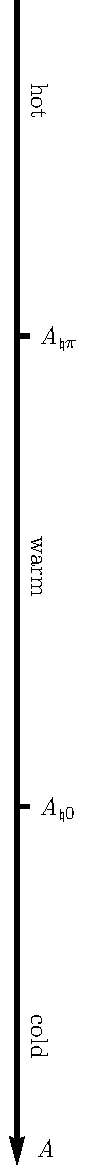
\includegraphics[height=13.6\textwidth]{bipolar-viable-arrow}
  \end{minipage}
  \begin{minipage}[b]{0.8\textwidth}
    \newcommand*{\legendtrimwidth}{0.03\textwidth}
    \newcommand*{\legendoffsetheight}{0.025\textwidth}
    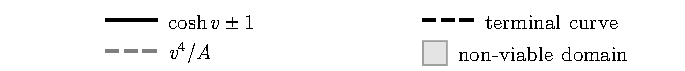
\includegraphics[
      width={\textwidth-\legendtrimwidth},
      trim={\legendtrimwidth} {-\legendoffsetheight} 0 0,
    ]{bipolar-viable-legend}
    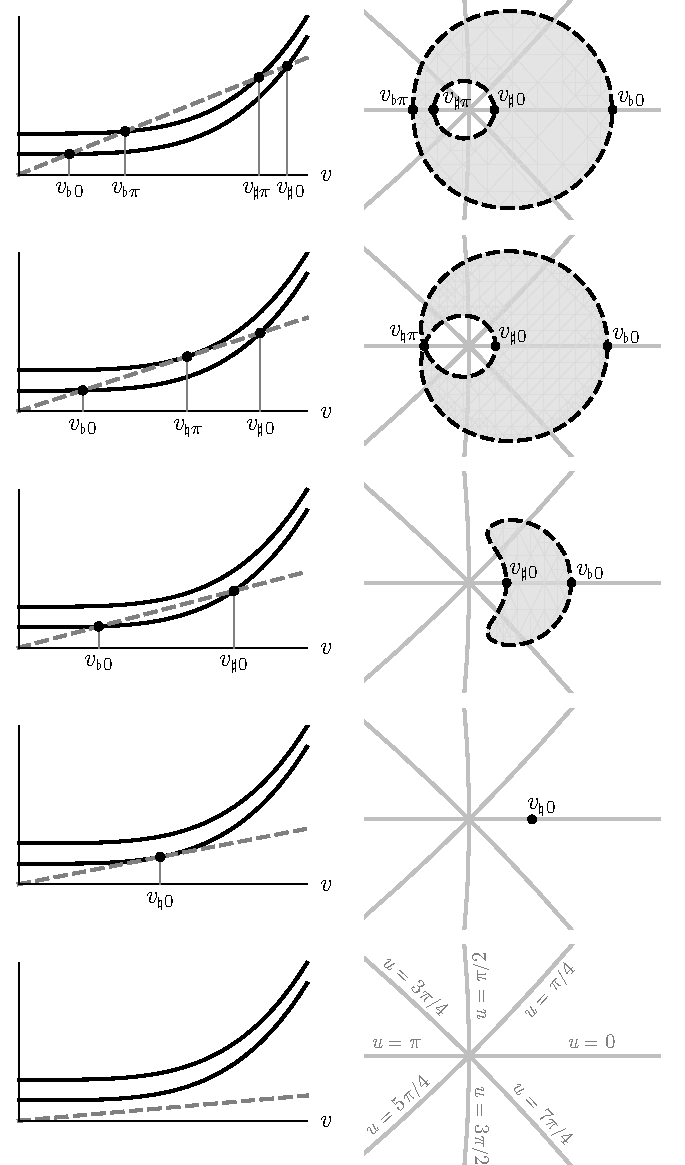
\includegraphics[width=\textwidth]{bipolar-viable}
  \end{minipage}
  \caption{
    Critical terminal points and non-viable domain~$\Phi < 0$
    for the known solution~(\ref{eq:bipolar-scaled-laplace-solution})
    and viability function~(\ref{eq:bipolar-viability-function}),
    as $A$~increases.
    In the right-hand column,
    the $u$-contours~\figurestyle{grey curves} meet
    at the positive singularity~$v = +\infty$.
  }
  \label{fig:bipolar-viable}
\end{figure}

Each of~(\ref{eq:bipolar-critical-terminal-point-pi})
and~(\ref{eq:bipolar-critical-terminal-point-0})
has zero to two roots
(ignoring~$v = 0$ for~(\ref{eq:bipolar-critical-terminal-point-0}))
depending on the size of the dimensionless group~$A$,
leading to five cases for the number of critical terminal points
and the geometry of the viable domain
(Figure~\ref{fig:bipolar-viable}):

\subsection{Five cases}
\label{sec:bipolar.viable.cases}

\begin{enumerate}
  \item
    \term{Hot regime}, $A < A_{\nat \pi}$:
    Both equations have two roots:
    $v_{\flat \pi}$ and~$v_{\sharp \pi}$
    for~(\ref{eq:bipolar-critical-terminal-point-pi})
    and
    $v_{\flat 0}$ and~$v_{\sharp 0}$
    for~(\ref{eq:bipolar-critical-terminal-point-0}),
    with~$v_{\flat 0} < v_{\flat \pi} < v_{\sharp \pi} < v_{\sharp 0}$.
    Thus there are four critical terminal points,
    having bipolar coordinates~$(0, v_{\flat 0})$, $(\pi, v_{\flat \pi})$,
    $(\pi, v_{\sharp \pi})$, and~$(0, v_{\sharp 0})$.
    The non-viable domain forms an avocado-like moat
    which surrounds an inner viable island
    (containing the singularity~$v = +\infty$)
    and is surrounded by an outer viable mainland.
  \item
    \term{Hot-to-warm transition}, $A = A_{\nat \pi}$:
    The two roots of~(\ref{eq:bipolar-critical-terminal-point-pi})
    merge together
    and the non-viable moat is pincered along~$u = \pi$,
    leaving the three critical terminal points~$(0, v_{\flat 0})$,
    $(\pi, v_{\nat \pi})$, and~$(0, v_{\sharp 0})$.
    The inner viable island and the outer viable mainland
    touch at the second of these.
  \item
    \term{Warm regime}, $A_{\nat \pi} < A < A_{\nat 0}$:
    The remaining root of~(\ref{eq:bipolar-critical-terminal-point-pi})
    disappears
    and the inner viable island is now robustly connected
    to the outer viable mainland.
    Equation~(\ref{eq:bipolar-critical-terminal-point-0}) still has two roots,
    corresponding to the two critical terminal points~%
      $(0, v_{\flat 0})$ and~$(0, v_{\sharp 0})$.
    The non-viable domain is now a crescent-shaped lake.
  \item
    \term{Warm-to-cold transition}, $A = A_{\nat 0}$:
    The two roots of~(\ref{eq:bipolar-critical-terminal-point-0})
    merge together
    and the non-viable lake dries up completely.
    The entire plane is viable,
    though a single (isolated) critical terminal point still exists
    at~$(0, v_{\nat 0})$.
  \item
    \term{Cold regime}, $A > A_{\nat 0}$:
    The remaining root of~(\ref{eq:bipolar-critical-terminal-point-0})
    disappears.
    The entire plane is viable,
    and there are no critical terminal points left.
\end{enumerate}
The two transition cases occur
when~(\ref{eq:bipolar-critical-terminal-point-pi})
and~(\ref{eq:bipolar-critical-terminal-point-0})
each have a merging of roots,
at the special values of~$A$
for which the curves~$\cosh v \pm 1$ and~$v^4 / A$
touch tangentially,
given by the extra condition
\begin{equation}
  \sinh v - \frac{4 v^3}{A} = 0.
  \label{eq:bipolar-critical-terminal-point-transition}
\end{equation}
Note how this accounts for the situation in which
the terminal curve has an indeterminate local tangent
in equation~(\ref{eq:bipolar-terminal-curve-implicit-derivative}).
By numerically solving each of~(\ref{eq:bipolar-critical-terminal-point-pi})
and~(\ref{eq:bipolar-critical-terminal-point-0})
in conjunction with the tangency condition~%
  (\ref{eq:bipolar-critical-terminal-point-transition}),
the values of~$A$ for the two transitions are determined to be
\begin{align}
  A_{\nat \pi} &= 9.06433 \eqnspace \text{hot-to-warm},
    \label{eq:bipolar-transition-a-hot-to-warm}
    \\
  A_{\nat 0} &= 9.76206 \eqnspace \text{warm-to-cold}.
    \label{eq:bipolar-transition-a-warm-to-cold}
\end{align}

\section{Boundary tracing}
\label{sec:bipolar.tracing}

In this section we write down the boundary tracing ODE
and determine the class of convex domains which can be constructed.

\subsection{Candidate boundaries}
\label{sec:bipolar.tracing.candidates}

\begin{figure}
  \newcommand*{\subfigurewidth}{0.45\textwidth}
  \newcommand*{\subfigureoffsettop}{0.08\textwidth}
  \newcommand*{\subfigureoffsetbottom}{0.04\textwidth}
  \centering
  \begin{subfigure}{\subfigurewidth}
    \centredfigurecontent[
      trim=0 {\subfigureoffsetbottom} 0 0,
    ]{bipolar-traced-boundaries-hot}{Hot regime}
  \end{subfigure}
  \hfill
  \begin{subfigure}{\subfigurewidth}
    \centredfigurecontent[
      trim=0 {\subfigureoffsetbottom} 0 0,
    ]{bipolar-traced-boundaries-warm}{Warm regime}
  \end{subfigure}
  
  \begin{subfigure}{\subfigurewidth}
    \centredfigurecontent[
      trim=0 {\subfigureoffsetbottom} 0 {-\subfigureoffsettop},
    ]{bipolar-traced-boundaries-cold}{Cold regime}
  \end{subfigure}
  \caption{
    Traced boundaries obtained by integrating~%
      (\ref{eq:bipolar-tracing-ode-coordinate-parametrisation-v}).
  }
  \label{fig:bipolar-traced-boundaries}
\end{figure}

Using~(\ref{eq:bipolar-gradient-u-component})
through~(\ref{eq:bipolar-viability-function}),
the boundary tracing ODE~(\ref{eq:tracing-ode-coordinate-parametrisation-v})
becomes
\begin{important}{equation}
  \tder{v}{u} =
    \pm
    \frac{A}{v^4}
    \sqrt{
      \roundbr[\bulkysize]{\cosh v - \cos u}^2 - \frac{v^8}{A^2}
    },
  \label{eq:bipolar-tracing-ode-coordinate-parametrisation-v}
\end{important}
which cannot be integrated analytically.
Traced boundaries determined by numerical integration
from starting points in the viable domain
are shown in Figure~\ref{fig:bipolar-traced-boundaries}.

Like the line-source case in Section~\ref{sec:polar.tracing},
the two branches of traced boundaries are segregated
by the sign of~$\td v / {\td u}$,
with the upper branch spiralling inwards
and the lower branch spiralling outwards
as one travels anticlockwise
around the singularity~$v = +\infty$.
Again, any physically sensible radiation--conduction domain
must completely surround the heat-supplying singularity without touching it,
and therefore we seek closed curves surrounding the singularity,
made from patching together the traced boundaries
given by~(\ref{eq:bipolar-tracing-ode-coordinate-parametrisation-v}).
Using similar arguments to those in Section~\ref{sec:polar.tracing},
we conclude that a necessary (but not sufficient) condition
for the convexity of the sought-after closed curve
is for it to have an upper-to-lower branch switch
at an hyperbolic critical terminal point.

\begin{figure}
  \newcommand*{\subfigurewidth}{0.35\textwidth}
  \newcommand*{\subfigureoffsetbottom}{0.08\textwidth}
  \centering
  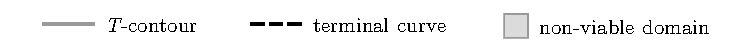
\includegraphics[
    width=0.85\textwidth,
    trim=0 -5 0 0,
  ]{bipolar-critical-terminal-points-legend}
  
  \hspace*{\fill}
  \begin{subfigure}{\subfigurewidth}
    \centredfigurecontent[
    ]{bipolar-critical-terminal-points-hot}{Hot regime}
  \end{subfigure}
    \hfill
  \begin{subfigure}{\subfigurewidth}
    \centredfigurecontent[
    ]{bipolar-critical-terminal-points-warm_hot}{Hot-to-warm transition}
  \end{subfigure}
  \hspace*{\fill}
  
  \hspace*{\fill}
  \begin{subfigure}{\subfigurewidth}
    \centredfigurecontent[
      trim=0 {\subfigureoffsetbottom} 0 0,
    ]{bipolar-critical-terminal-points-warm}{Warm regime}
  \end{subfigure}
    \hfill
  \begin{subfigure}{\subfigurewidth}
    \centredfigurecontent[
      trim=0 {\subfigureoffsetbottom} 0 0,
    ]{bipolar-critical-terminal-points-cold_warm}{Warm-to-cold transition}
  \end{subfigure}
  \hspace*{\fill}
  \caption{
    Local $T$-contour through each critical terminal point.
  }
  \label{fig:critical-terminal-points}
\end{figure}

The nature of the up to four critical terminal points that exist
can be determined by inspecting Figure~\ref{fig:critical-terminal-points}.
We see that those lying on the segment~$u = \pi$
(to the left of the singularity)
are of elliptic type,
as the local $T$-contour lies on the non-viable side of the terminal curve.
Only the critical terminal points lying on the segment~$u = 0$
(to the right of the singularity)
are of hyperbolic type,
and it is from these points that we might construct convex domains.
Explicitly, we have two hyperbolic critical terminal points~%
$(u, v) = (0, v_{\flat 0})$ and~$(u, v) = (0, v_{\sharp 0})$
for~$0 < A < A_{\nat 0}$ (the hot regime through to the warm regime),
which merge to become the single point~$(u, v) = (0, v_{\nat 0})$
at~$A = A_{\nat 0}$ (the warm-to-cold transition),
which then disappears for~$A > A_{\nat 0}$ (the cold regime).

\begin{figure}
  \centering
  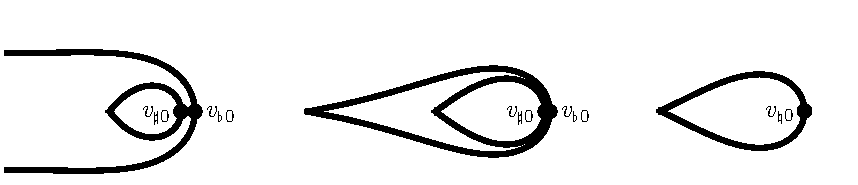
\includegraphics[width=\textwidth]{bipolar-candidates}
  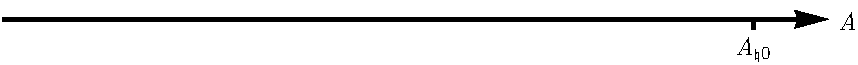
\includegraphics[width=\textwidth]{bipolar-candidates-arrow}
  \caption{
    Inner~($v_{\sharp 0}$) and outer~($v_{\flat 0}$) candidate boundaries,
    as $A$~increases.
    The two candidate boundaries become one at~$A = A_{\nat 0}$.
  }
  \label{fig:bipolar-candidates}
\end{figure}

We may therefore construct (up to) two \term{candidate boundaries}
whenever~$0 < A \le A_{\nat 0}$,
as shown in Figure~\ref{fig:bipolar-candidates}.
An \term{outer candidate boundary} is constructed
by performing an upper-to-lower branch switch at~$(0, v_{\flat 0})$,
i.e.~by taking the upper branch for~$-\pi < u \le 0$
and joining it to the lower branch for~$0 \le u < \pi$.
An \term{inner candidate boundary} is produced likewise
from the point~$(0, v_{\sharp 0})$.
The two boundaries merge together
when $v_{\flat 0}$ and~$v_{\sharp 0}$ merge
at the warm-to-cold transition~$A = A_{\nat 0}$.

The inner candidate boundary forms a closed loop
and appears to be convex over the entire interval~$0 < A \le A_{\nat 0}$.
The outer candidate boundary only forms a closed loop
if $A$~is sufficiently large,
but in the next section we show that this is irrelevant
because the outer candidate boundary is always non-convex.

\subsection{Convexity of the candidate boundaries}
\label{sec:bipolar.tracing.convex}

We first consider the inner candidate boundary,
which always forms a closed loop
by way of its two branches meeting in a corner
at~$(u, v) = (\mp\pi, v_\End)$ on the left
(Figure~\ref{fig:bipolar-inner-candidate}).
While this boundary appears to be convex for all~$A \le A_{\nat 0}$,
we cannot be certain until a global curvature analysis is performed
like that of Section~\ref{sec:polar.convex.beyond}.

\begin{figure}
  \centredfigurecontent[width=0.45\textwidth]{%
    bipolar-inner-candidate%
  }{
    Bipolar coordinates of the left-hand and right-hand extremities
    of an inner candidate boundary.
  }
\end{figure}

From the coordinate transformations
we obtain the orthonormal basis vectors
\begin{align}
  \basisvec{u} &= -\scalefac S \basisvec{x} + \scalefac C \basisvec{y},
    \label{eq:u-basis-vector-bipolar} \\
  \basisvec{v} &= -\scalefac C \basisvec{x} - \scalefac S \basisvec{y},
    \label{eq:v-basis-vector-bipolar}
\end{align}
where
\begin{align}
  S &= \sin u \sinh v,
    \label{eq:bipolar-abbreviation-s} \\
  C &= \cos u \cosh v - 1,
    \label{eq:bipolar-abbreviation-c}
\end{align}
and $\scalefac$~is the dimensionless scale factor~%
  (\ref{eq:dimensionless-scale-factor-bipolar}).
We consider a curve parametrised in the form~$v = v (u)$,
and let primes denote $u$-differentiation.
After some algebra, we find that
the basis vectors~(\ref{eq:u-basis-vector-bipolar})
and~(\ref{eq:v-basis-vector-bipolar})
change according to
\begin{align}
  (\basisvec{u})'
  &= -\scalefac^2 C D \basisvec{x} - \scalefac^2 S D \basisvec{y}
  = +\scalefac D \basisvec{v},
    \label{eq:u-basis-vector-u-derivative-bipolar} \\
  (\basisvec{v})'
  &= +\scalefac^2 S D \basisvec{x} - \scalefac^2 C D \basisvec{y}
  = -\scalefac D \basisvec{u},
    \label{eq:v-basis-vector-u-derivative-bipolar}
\end{align}
where
\begin{equation}
  D = \sinh v - v' \sin u.
  \label{eq:bipolar-abbreviation-d}
\end{equation}
Now, from the differential displacement
\begin{equation}
  \td\positionvec =
    \scalefac \td u \basisvec{u} + \scalefac \td v \basisvec{v},
  \label{eq:differential-displacement-bipolar}
\end{equation}
we have the velocity
\begin{equation}
  \positionvec' = \tder{\positionvec}{u} =
    \scalefac \basisvec{u} + \scalefac v' \basisvec{v}.
  \label{eq:velocity-vector-bipolar-by-u}
\end{equation}
Taking another $u$-derivative,
and using~(\ref{eq:u-basis-vector-u-derivative-bipolar})
and~(\ref{eq:v-basis-vector-u-derivative-bipolar})
to simplify,
we obtain the acceleration
\begin{equation}
  \positionvec'' = \tder[2]{\positionvec}{u} =
    - \scalefac^2 (D v' + E) \basisvec{u}
    + \scalefac (v'' - \scalefac E v' + \scalefac D) \basisvec{v},
  \label{eq:acceleration-vector-bipolar-by-u}
\end{equation}
where
\begin{equation}
  E = v' \sinh v + \sin u.
  \label{eq:bipolar-abbreviation-e}
\end{equation}
A quantity having the same sign changes as curvature is therefore
\begin{equation}
  \kappa = \basisvec{z} \dotp (\positionvec' \crossp \positionvec'') =
    \scalefac^3
    \squarebr*{D \roundbr*{1 + {v'}^2} + \frac{v''}{\scalefac}}.
  \label{eq:kappa-bipolar-by-u}
\end{equation}
Inspecting
Figures~\ref{fig:bipolar-candidates} and~\ref{fig:bipolar-inner-candidate}
once more,
we note again that
the inner candidate boundary appears to be always convex.
Certainly the rotund right-hand end is convex.
However, while the tip at the left-hand end looks to be a convex corner,
there remains the possibility
that it could actually be a non-convex spike,
similar to Figure~\hyperref[fig:plane-domains]{\ref*{fig:plane-domains}c}
(although much more subtle).
To test this,
we evaluate~(\ref{eq:kappa-bipolar-by-u}),
first using the traced boundary derivative~%
  (\ref{eq:bipolar-tracing-ode-coordinate-parametrisation-v})
for~$v'$,
and then substituting~$u = \mp\pi$
(which is the location of the tip for each branch).
We obtain
\begin{equation}
  \eval*{\kappa}_{u = \mp\pi} =
    \frac{2 A^2}{v^9}
    \roundbr*{-2 + v \tanh\frac{v}{2}},
    \label{eq:bipolar-traced-boundary-kappa-bipolar-by-u-tip}
\end{equation}
which changes sign at the positive solution to the transcendental equation
\begin{equation}
  \frac{v}{2} \tanh\frac{v}{2} = 1,
\end{equation}
numerically
\begin{equation}
  v = v_\infl = 2.39936.
  \label{eq:bipolar-v-inflection-tip}
\end{equation}
The inner candidate boundary will therefore be convex
if and only if its tip at the left-hand end~$(u, v) = (\mp\pi, v_\End)$
either coincides with or lies to the right of~$(u, v) = (\mp\pi, v_\infl)$.
Algebraically, we will have convexity if and only if~$v_\End \ge v_\infl$.
We see from Figure~\ref{fig:bipolar-candidates}
that the tip is furthest to the left when~$A = A_{\nat 0}$
(when the inner and outer candidates merge),
and in this worst-case scenario
the tip coordinate computes to~$v_\End = 2.20618$,
which is \emph{less than}
the critical value~(\ref{eq:bipolar-v-inflection-tip}).
It follows that the inner candidate boundary is in fact non-convex for
\begin{equation}
  A_\infl < A \le A_{\nat 0},
  \label{eq:bipolar-inner-candidate-non-convex-a-interval}
\end{equation}
where the lower bound~$A_\infl$ is the value of~$A$ at which
\begin{equation}
  v_\End = v_\infl,
  \label{eq:bipolar-inner-candidate-a-inflection-equation}
\end{equation}
corresponding to inflection occurring exactly at the tip.
Using the bisection algorithm we obtain
\begin{equation}
  A_\infl = 9.76036,
  \label{eq:bipolar-inner-candidate-a-inflection}
\end{equation}
which is extremely close to the upper value~$A_{\nat 0} = 9.76206$:
indeed the width of the interval~%
  (\ref{eq:bipolar-inner-candidate-non-convex-a-interval})
is an exceedingly minuscule~$1.7 \times 10^{-3}$.
It is pure coincidence that
among the entire interval~$0 < A \le A_{\nat 0}$
of inner candidate boundaries,
such a tiny fraction of them should be non-convex.
While this is most remarkable from a theoretical perspective,
we note that there is little significance in practice,
as the amount of self-viewing radiation is exceptionally tiny.

For the outer candidate boundary,
we return again to Figure~\ref{fig:bipolar-candidates}.
First we rule out the candidates with $A$~too small,
as these do not form a closed loop.
Of the remaining outer candidate boundaries
(which do form a closed loop),
we observe that the left-hand tip at best
coincides with the tip of the $A = A_{\nat 0}$~boundary
(when the inner and outer candidates merge).
As we have just seen from the analysis of the inner candidate,
this $A = A_{\nat 0}$~boundary is non-convex.
Hence, the outer candidate boundary
never forms a convex closed loop.

While it is possible to quantify the amount of self-viewing radiation
to determine non-convex yet practical domains
(both for the minuscule continuum~%
  (\ref{eq:bipolar-inner-candidate-non-convex-a-interval})
of inner candidate boundaries
and for the outer candidate boundaries that form a closed loop),
we omit such an analysis here
for the same reasons as given in Section~\ref{sec:polar.convex.self-viewing}.

\subsection{Numerical verification}
\label{sec:bipolar.tracing.verification}

\begin{figure}[b]
  \centering
  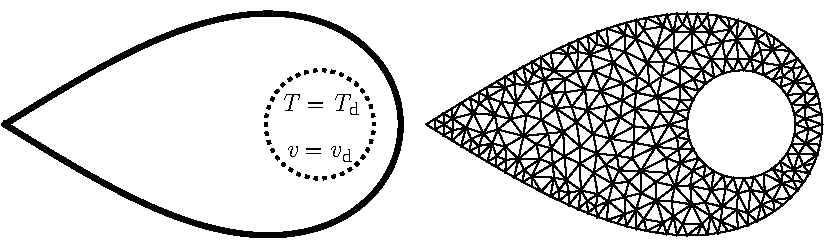
\includegraphics[width=0.9\textwidth]{bipolar-verification-domain-mesh}
  
\includegraphics[width=\textwidth]{line-verification-domain-mesh-legend}
  \caption{
    Selected domain and finite element mesh for numerical verification.
  }
  \label{fig:bipolar-verification-domain-mesh}
\end{figure}

\begin{figure}
  \centredfigurecontent[width=0.52\textwidth]{%
    bipolar-inner-candidate-with-circle%
  }{
    Circle~$v = v_{\sharp 0}$~\figurestyle{grey},
    which touches the inner candidate boundary~\figurestyle{black}
    at the critical terminal point~$(u, v) = (0, v_{\sharp 0})$.
  }
\end{figure}

For numerical verification using finite elements,
we consider the conduction--radiation domain shown
in Figure~\ref{fig:bipolar-verification-domain-mesh}.
The radiation boundary is the inner candidate boundary for~$A = 9.76$.
The heat-supplying singularity~$v = +\infty$
we have replaced with an equivalent Dirichlet condition~$T = T_\dir$
along a circle~$v = v_\dir$,
where~$T_\dir = v_\dir$
per the known solution~(\ref{eq:bipolar-scaled-laplace-solution}).
It is necessary to choose~$v_\dir > v_{\sharp 0}$
so that the Dirichlet boundary is a strictly interior one,
since the circle~$v = v_{\sharp 0}$ touches
the right-hand end of the radiation boundary
at the critical terminal point~$(0, v_{\sharp 0})$
(Figure~\ref{fig:bipolar-inner-candidate-with-circle}).
Here we have selected~$v_\dir = 1.1 v_{\sharp 0} = 4.26$,
so that the constant-temperature boundary
of Figure~\ref{fig:bipolar-verification-domain-mesh}
is a circle of radius~$0.028$.

We again use \software{Mathematica}'s \code{NDSolve\`{}FEM\`{}},
generating a mesh with approximately 500~triangular elements.
The relevant conduction--radiation BVP is solved numerically,
consisting of Laplace's equation in the interior,
the radiation condition~(\ref{eq:bipolar-scaled-radiation-boundary-condition})
on the external boundary,
and the aforesaid Dirichlet condition on the interior boundary.
Comparing the resulting numerical solution
to the known exact solution~(\ref{eq:bipolar-scaled-laplace-solution}),
we find that the maximum relative error throughout the mesh
is of the order~$10^{-3}$
(Figure~\ref{fig:bipolar-verification}).

\begin{figure}
  \newcommand*{\subfigurewidth}{0.42\textwidth}
  \centering
  \hspace*{\fill}
  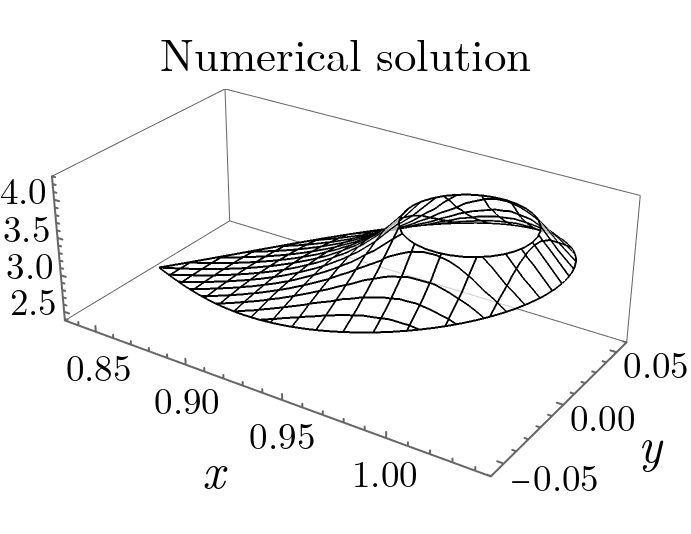
\includegraphics[width=\subfigurewidth]{bipolar-verification-solution}
    \hfill
  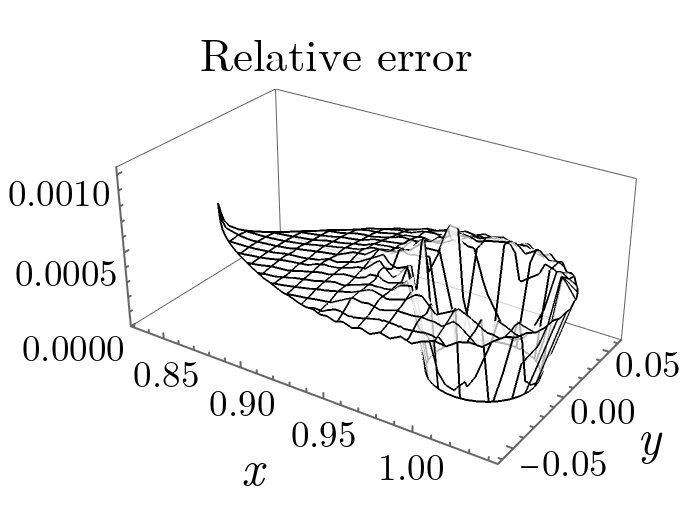
\includegraphics[width=\subfigurewidth]{bipolar-verification-relative-error}
  \hspace*{\fill}
  \caption{
    Numerical verification.
  }
  \label{fig:bipolar-verification}
\end{figure}

\section{Physical range}
\label{sec:bipolar.physical}

In this section, we determine for various quantities
the physical range that can be achieved over the continuum
\begin{equation}
  0 < A \le A_{\nat 0}
  \label{eq:bipolar-inner-candidate-existence-interval}
\end{equation}
of inner candidate boundaries.
For the purposes of this analysis,
we shall ignore the issue of non-convexity
in the minute subinterval~%
  (\ref{eq:bipolar-inner-candidate-non-convex-a-interval}),
with the special value~$A_{\nat 0}$
serving as an algebraically convenient approximation
for the upper limit~$A_\infl$ of convexity.
We return here to unscaled variables,
restoring the \scalingmarks{} which were dropped
from (\ref{eq:bipolar-scaled-radiation-boundary-condition})~onwards.

\subsection{Asymmetry}
\label{sec:bipolar.physical.asymmetry}

Inspecting the inner candidate boundaries
of Figure~\ref{fig:bipolar-candidates},
we see that an increase in the dimensionless group~$A$
results in an elongation of the characteristic teardrop shape.
This makes sense physically.
The bipolar solution~(\ref{eq:bipolar-laplace-solution})
to Laplace's equation
arises from the superposition of equal and opposite line sources
at~$(x, y) = (\pm a, 0)$,
so we may think of it as a perturbation of
the radial line-source solution~(\ref{eq:line-laplace-solution})
caused by the introduction of an opposite line source at distance~$2 a$.
Since the dimensionless group~$A$
is inversely proportional to the length scale~$a$
(see~(\ref{eq:bipolar-dimensionless-group})),
an increase in~$A$ brings the second line source (which is cold)
closer to the first line source (which is hot),
thus increasing the amount of asymmetry.

It is no coincidence that we have a non-viable moat
separating an inner viable island from an outer viable mainland,
both for the line-source solution of Chapter~\ref{ch:polar}
and for the present bipolar solution, when $A$ is sufficiently small.
The limiting case of~$A = 0$
corresponds to the second line source being infinitely far removed,
i.e.~a reduction to the purely radial case.

The inner candidate boundary for the bipolar solution
is in fact a deformed version
of the trivial circular traced boundary~($r = r_\flat$)
that exists on the inner viable island,
in the hot regime of the line-source solution
(Section~\ref{sec:polar.tracing.hot}).
In the limiting $A = 0$~case,
the inner candidate boundary would be a circle
centred on the singularity~$v = +\infty$,
but for~$A > 0$,
the presence of the negative singularity
causes the inner candidate boundary to deviate
from perfectly circularity.
The amount of asymmetry may be quantified
through the ratio of distances from
the ideal centre~$(x, y) = (+a, 0)$
(which is the singularity~$v = +\infty$)
to each of the left-hand and right-hand extremities
(which have bipolar coordinates $(\mp\pi, v_\End)$ and~$(0, v_{\sharp 0})$
respectively; see Figure~\ref{fig:bipolar-inner-candidate}).
Thus
\begin{align*}
  \textq{Asymmetry}
  &=
    \frac{a - x_\End}{x_{\sharp 0} - a}
      \\[\tallspace]
  &=
    \frac{
      1 - \sinh v_\End / (\cosh v_\End - \cos(\mp\pi))
    }{
      \sinh v_{\sharp 0} / (\cosh v_{\sharp 0} - \cos 0) - 1
    }
      \\[\tallspace]
  &=
    \frac{\exp v_{\sharp 0} - 1}{\exp v_\End + 1}.
    \yesnumber
    \label{eq:bipolar-inner-candidate-asymmetry}
\end{align*}
The asymmetry will only become significant
if the negative line source has been brought
sufficiently close to the positive one.
From Figure~\ref{fig:bipolar-inner-candidate-asymmetry}
we see that this only occurs towards the colder end of the warm regime.

\begin{figure}
  \centredfigurecontent[width=0.6\textwidth]{%
    bipolar-inner-candidate-asymmetry%
  }{
    Asymmetry~(\ref{eq:bipolar-inner-candidate-asymmetry})
    of the inner candidate boundary,
    as $A$~increases.
    No inner candidate boundary exists
    in the cold regime~($A > A_{\nat 0}$).
  }
\end{figure}

\subsection{Temperature}
\label{sec:bipolar.physical.temperature}

Here we perform a similar analysis
to Section~\ref{sec:polar.physical.temperature},
to determine the physical temperatures that can be realised
by inner candidate boundaries of a prescribed size.
For simplicity,
we take the radius of the circle~$v = v_{\sharp 0}$
(Figure~\ref{fig:bipolar-inner-candidate-with-circle})
as our fixed reference length.
From~(\ref{eq:bipolar-circle-v})
we see that this radius is given by
\begin{equation}
  r_{\sharp 0} = a \csch v_{\sharp 0},
  \label{eq:bipolar-r-sharp-0}
\end{equation}
so that the length scale (intrinsic to the bipolar coordinate system) is
\begin{equation}
  a = r_{\sharp 0} \sinh v_{\sharp 0}.
  \label{eq:bipolar-length-scale-in-terms-of-r-sharp-0}
\end{equation}
By construction, the bipolar coordinate~$v_{\sharp 0}$
is a root of the equation~(\ref{eq:bipolar-critical-terminal-point-0})
for critical terminal points along~$u = 0$;
therefore we have
\begin{equation}
  A = \frac{{v_{\sharp 0}}^4}{\cosh v_{\sharp 0} - 1}.
  \label{eq:bipolar-dimensionless-group-in-terms-of-r-sharp-0}
\end{equation}
After rearranging~(\ref{eq:bipolar-dimensionless-group}) for~$T_0$,
we may use~(\ref{eq:bipolar-length-scale-in-terms-of-r-sharp-0})
and~(\ref{eq:bipolar-dimensionless-group-in-terms-of-r-sharp-0})
to obtain
\begin{equation}
  T_0 =
    \roundbr*{
      \frac{
        \cosh v_{\sharp 0} - 1
      }{
        c r_{\sharp 0} {v_{\sharp 0}}^4 \sinh v_{\sharp 0}
      }
    }^{1/3}
  \label{eq:bipolar-temperature-scale-in-terms-of-r-sharp-0}
\end{equation}
for the temperature scale
of the known solution~(\ref{eq:bipolar-laplace-solution}).
It follows that the physical temperature
along the reference circle~$v = v_{\sharp 0}$
is
\begin{align*}
  T_{\sharp 0}
  &= T_0 \cdot v_{\sharp 0} \\
  &=
    \roundbr*{
      \frac{
        \cosh v_{\sharp 0} - 1
      }{
        c r_{\sharp 0} v_{\sharp 0} \sinh v_{\sharp 0}
      }
    }^{1/3}
    \\
  &=
    \roundbr*{
      \frac{\omega (v_{\sharp 0})}{c r_{\sharp 0}}
    }^{1/3},
    \yesnumber
    \label{eq:bipolar-t-sharp-0-in-terms-of-r-sharp-0}
\end{align*}
where $\omega$~is the dimensionless auxiliary function
\begin{equation}
  \omega (v) = \frac{\cosh v - 1}{v \sinh v}
  \label{eq:bipolar-auxiliary-function}
\end{equation}
shown in Figure~\ref{fig:bipolar-auxiliary-function}.

\begin{figure}
  \centredfigurecontent[width=0.55\textwidth]{%
    bipolar-auxiliary-function%
  }{
    Auxiliary function~(\ref{eq:bipolar-auxiliary-function}).
  }
\end{figure}

Now, as the dimensionless group~$A$
runs through the interval~%
  (\ref{eq:bipolar-inner-candidate-existence-interval})
of all inner candidate boundaries,
i.e.~from the limiting extreme~$A = 0$ of the hot regime
up to the warm-to-cold transition~$A = A_{\nat 0} = 9.76206$,
the quantity~$v_{\sharp 0}$ decreases from infinity
down to the transition value~$v_{\nat 0} = 3.83002$;
this can be seen from the left-hand column
of Figure~\ref{fig:bipolar-viable}.
It can be shown that $\omega$~is a decreasing function,
whence we have
\begin{equation}
  \omega (\infty) < \omega (v_{\sharp 0}) \le \omega (v_{\nat 0}).
  \label{eq:bipolar-inner-candidate-omega-interval}
\end{equation}
The upper bound may in fact be simplified to~$1/4$,%
\footnote{
  This would not have happened
  had we chosen $A_\infl$ instead of the special value~$A_{\nat 0}$
  for the upper bound of the interval~%
  (\ref{eq:bipolar-inner-candidate-existence-interval}).
}
so we have
\begin{equation}
  0 < \omega (v_{\sharp 0}) \le 1/4.
  \label{eq:bipolar-inner-candidate-omega-interval-evaluated}
\end{equation}
Therefore,
the unscaled temperature~(\ref{eq:bipolar-t-sharp-0-in-terms-of-r-sharp-0})
spans the interval
\[
  0
    <
  T_{\sharp 0}
    \le
  \roundbr*{\frac{1}{4 c r_{\sharp 0}}}^{1/3},
\]
or
\begin{equation}
  0
    <
  T_{\sharp 0}
    \le
  \frac{1}{2^{2/3}}
  \roundbr*{\frac{\conduc}{\emiss \stefan r_{\sharp 0}}}^{1/3}.
  \label{eq:bipolar-inner-candidate-t-sharp-0-interval}
\end{equation}
It is interesting to note that this interval
perfectly complements the analogous line-source result~%
  (\ref{eq:line-traced-boundary-hot-convex-t-sharp-interval}),
whose lower bound is precisely the upper bound here
(with $r_\sharp$ in place of~$r_{\sharp 0}$).
For the PVC parameter values
of Section~\ref{sec:polar.physical.temperature},
the interval~(\ref{eq:bipolar-inner-candidate-t-sharp-0-interval})
evaluates to $\SI{0}{\kelvin} < T_{\sharp 0} \le \SI{277}{\kelvin}$.

At first glance one is tempted to conclude that physically,
the introduction of a negative image source
has the effect of extending the interval of possible temperatures
down to absolute zero.
However, upon closer inspection we see that
the exact agreement between the bounds is in fact fortuitous,
as it is the \emph{lower} bound
of~(\ref{eq:bipolar-inner-candidate-t-sharp-0-interval})
which is realised
when the bipolar solution reduces to the line-source solution
at~$A = 0$.
The upper bound is instead realised at
the warm-to-cold transition~$A = A_{\nat 0}$.

While the perfect agreement between the temperature bounds is a coincidence,
there is still reason for them to be of similar magnitude.
The physical ranges of Section~\ref{sec:polar.physical}
(for the line-source solution)
were derived for convex domains
constructed on the outer viable mainland of the hot regime.
These convex domains were constructed
in Section~\ref{sec:polar.convex.construction}
by making protrusions from the outer terminal curve~$r = r_\sharp$.
The bipolar inner candidate boundaries here are an analogue
\emph{not} of those protrusions on the outer viable mainland,
but of the circular traced boundary~$r = r_\flat$,
which was the sole convex boundary of the inner viable island.
That boundary was not analysed further due to its trivial shape,
but one may show that its corresponding temperature interval
is precisely~(\ref{eq:bipolar-inner-candidate-t-sharp-0-interval})
with $r_\flat$ in place of~$r_{\sharp 0}$.
Thus, the true reason for the agreement between the temperature bounds
is the similarity
between the bipolar inner candidate
and the line-source inner circle~$r = r_\flat$.

\subsection{Power per unit length}
\label{sec:bipolar.physical.power}

Returning now to the bipolar inner candidate,
the rate at which heat is generated internally
(and thus expelled via radiation from the boundary)
is fixed by the strength of the singularity~$v = +\infty$,
corresponding to the positive term
of~(\ref{eq:bipolar-laplace-solution-terms}).
Physically this is identical
to the fundamental line-source~(\ref{eq:line-laplace-solution}),
so we again have~(\ref{eq:line-power-per-length-fundamental}), i.e.
\begin{equation}
  p = 2 \pi \conduc T_0,
  \label{eq:line-power-per-length-fundamental-repeat}
\end{equation}
for the power dissipated per unit length.
Using~(\ref{eq:bipolar-temperature-scale-in-terms-of-r-sharp-0}),
this becomes
\begin{align*}
  p
  &=
    2 \pi \conduc
    \roundbr*{
      \frac{
        \cosh v_{\sharp 0} - 1
      }{
        c r_{\sharp 0} {v_{\sharp 0}}^4 \sinh v_{\sharp 0}
      }
    }^{1/3}
      \\[\tallspace]
  &=
    \frac{2 \pi \conduc}{(c r_{\sharp 0})^{1/3}}
    \roundbr*{
      \frac{
        \omega (v_{\sharp 0})
      }{
        {v_{\sharp 0}}^3
      }
    }^{1/3}.
      \yesnumber
      \label{eq:bipolar-power-per-length}
\end{align*}
As before, $\omega (v_{\sharp 0})$~runs through the interval~%
  (\ref{eq:bipolar-inner-candidate-omega-interval-evaluated})
as $v_{\sharp 0}$~decreases from infinity down to~$v_{\nat 0} = 3.83002$.
Therefore we have the interval
\[
  0 < p \le
    \frac{2 \pi \conduc}{(c r_{\sharp 0})^{1/3}}
    \roundbr*{
      \frac{
        1/4
      }{
        {v_{\nat 0}}^3
      }
    }^{1/3}
\]
in power per unit length, or
\begin{equation}
  0 < p \le
    \frac{2^{1/3}}{v_{\nat 0}}
    \frac{\pi \conduc^{4/3}}{(\emiss \stefan r_{\sharp 0})^{1/3}},
\end{equation}
evaluating to $0 < p \le \SI{82}{\watt \per\metre}$
for the parameters from the PVC example
of Section~\ref{sec:polar.physical.temperature}.

Unlike the temperature interval~%
  (\ref{eq:bipolar-inner-candidate-t-sharp-0-interval}),
the upper bound here does not coincide exactly
with the lower bound of~%
  (\ref{eq:line-traced-boundary-hot-convex-power-per-length-interval})
for power per unit length in the line-source solution.
As noted in Section~\ref{sec:bipolar.physical.temperature},
perfect agreement would be coincidental,
but we should nevertheless expect a similar order of magnitude.
A quick calculation shows that the prefactor here is
\[
  \frac{2^{1/3}}{v_{\nat 0}} = 0.32896,
\]
a mere $\SI{4}{\percent}$~more than the prefactor
\[
  \frac{1}{2^{5/3}} = 0.31498
\]
for the lower bound of~%
  (\ref{eq:line-traced-boundary-hot-convex-power-per-length-interval}).

\section{Summary}
\label{sec:bipolar.summary}

In this chapter, we have used boundary tracing
to analyse the conduction--radiation problem
for the bipolar solution~(\ref{eq:bipolar-laplace-solution}).
After developing the bipolar coordinate system
from first principles
in order to better understand the physics,
we have determined how the critical terminal points merge and disappear
as the sole dimensionless group~(\ref{eq:bipolar-dimensionless-group})
increases.
Accordingly, we have identified five cases
for the topology of the viable domain,
being three regimes separated by two transitions.

A continuum of so-called inner candidate boundaries can be constructed,
which have the potential to represent convex conduction--radiation domains.
Through further analysis we have shown that
while the majority of these candidates are indeed convex,
a tiny fraction of them are actually self-viewing
(but to a degree that is likely negligible in practice).
The validity of the produced domains has been confirmed
by comparing finite element solutions for the conduction--radiation BVP
against the exact solution~(\ref{eq:bipolar-laplace-solution}).

Finally we have determined the physical ranges
for asymmetry, temperature, and power per unit length
that can be achieved
among candidate boundaries of a prescribed size;
moreover, we have reconciled these results
with those in Section~\ref{sec:polar.physical}
for the purely radial line-source solution,
which is a limiting case of the bipolar solution
when the negative image source is infinitely far removed.
